% ---------------------------------------------------------------------------- %
\begin{figure}
  \centering
	\subfigure[\label{fig:conclusions:end:1}]
	{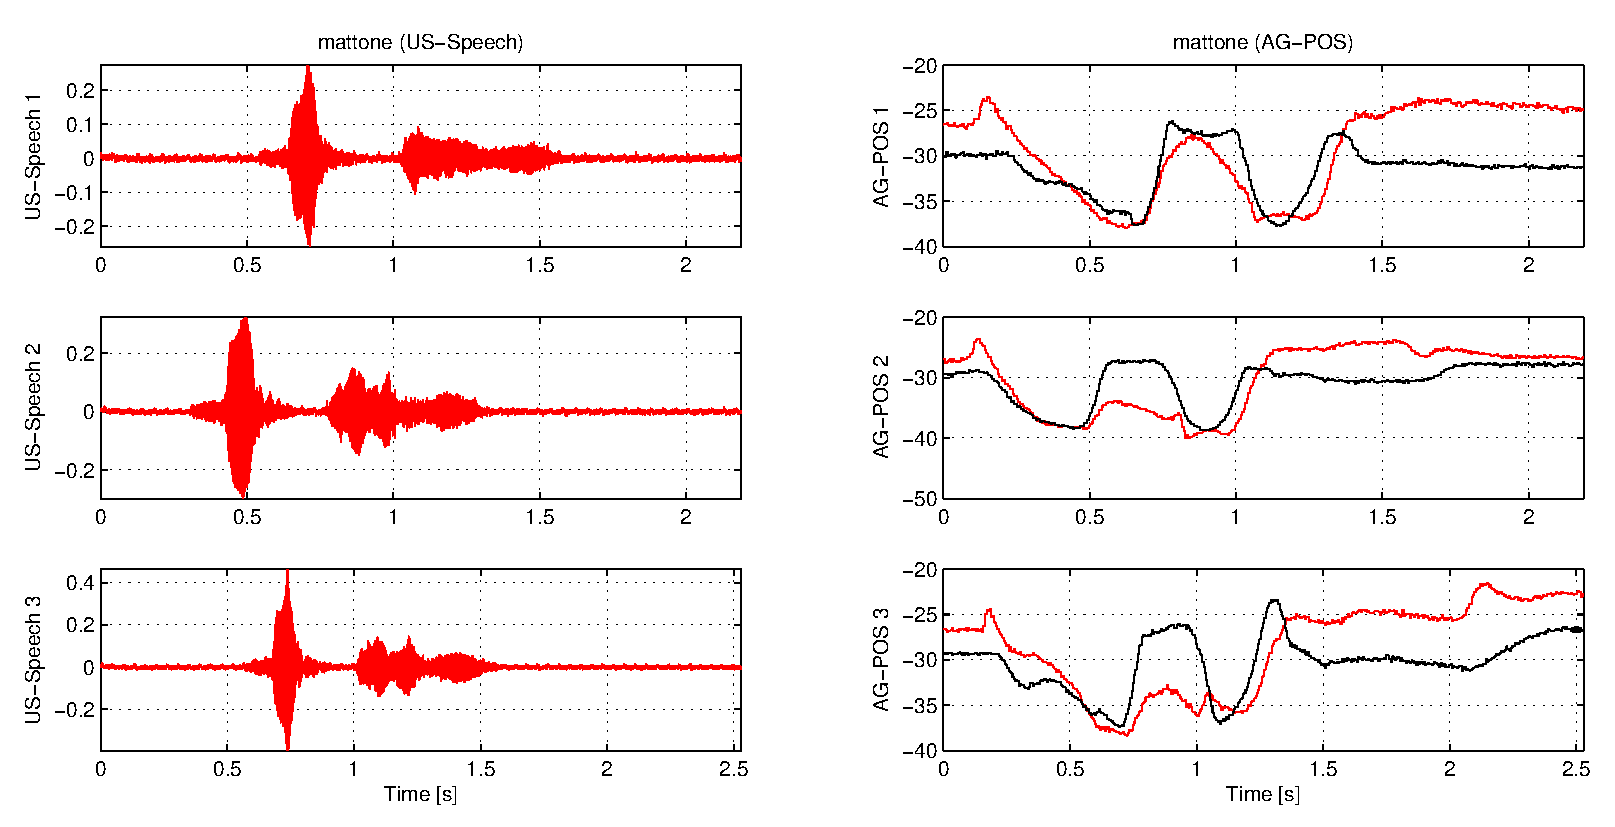
\includegraphics[width=\textwidth]{include/conclusions/images/end_same.eps}}
	
	\subfigure[\label{fig:conclusions:end:2}]
	{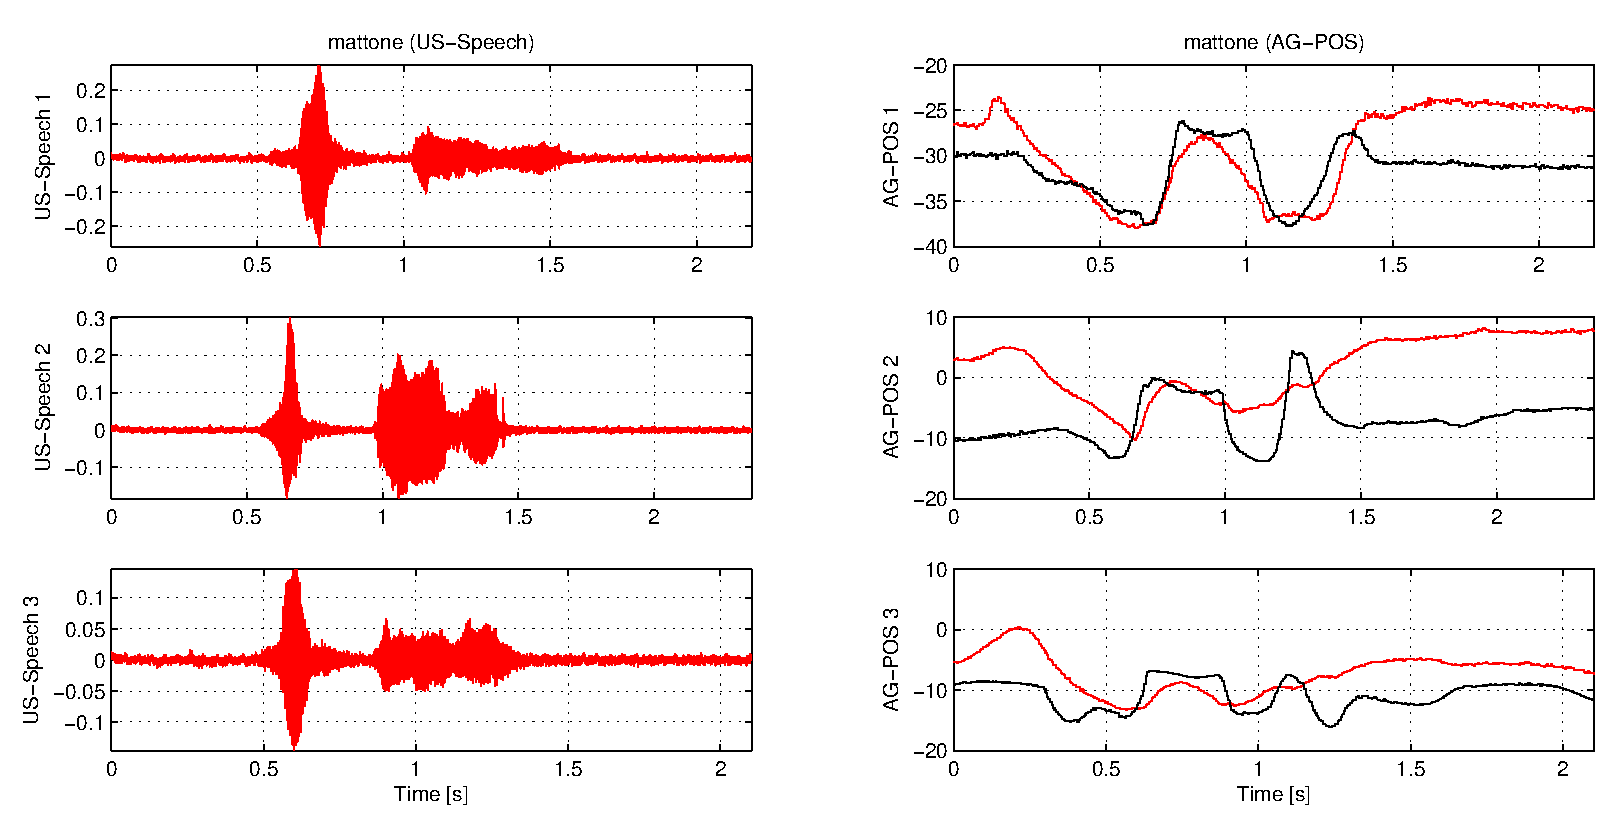
\includegraphics[width=\textwidth]{include/conclusions/images/end_diff.eps}}

	\caption[Speech signals and tongue vertical displacement]
	{\textbf{Speech signals and tongue vertical displacement}: (a) a subject
	(Subject 1) pronounces /mattone/ for three times. 
	(b) Three different subjects (Subjects 1, 4 and 5) pronounce /mattone/.
	For both panels: on the left, waveforms; on the right, vertical
	displacement (Z coordinate) of Sensor 3 (tongue tip, in red) and Sensor 1
	(tongue root, in black).
	The reader may be interested in looking at Figure~\ref{fig:experiments:map}
	and Table~\ref{tab:experiments:subjects} to obtain more details about 
	the positions of the sensors and subjects' age and gender.}
	\label{fig:conclusions:end}
\end{figure}
% ---------------------------------------------------------------------------- %
